Empezaremos mencionando y caracterizando algunas familias de grafos
para las que nuestra heurist\'ica golosa constructiva siempre encuentra
un resultado correcto, esto es, una clique de m\'axima frontera.

Teniendo en cuenta, como ya se menciono anteriormente, que la heur\'istica
empieza por uno de los nodos de mayor grado y en cada paso va 
agregando nodos que forman clique con los nodos actualmente escogidos
bajo la condici\'on de que el grado de los mismos sea mayor a dos veces
el tama\~no de la clique actual (de estos candidatos, tambi\'en elige
uno de los de mayor grado). Tenemos lo siguiente:

En todos los casos en los que hay varios candidatos para agregar a la
clique con el mismo grado (en particular el primero) la heur\'istica
puede proporcionar el resultado incorrecto, dado que el algoritmo
elige determin\'isticamente uno de los candidatos mientras que la 
entrada es aleatoria (la idea es poder resolver el problema para
cualquier grafo de entrada), veremos a continuaci\'on que excepto
en casos muy particulares, grafos isomorfos cuyas matrices de adyacencia
son distintas pueden, al ser sometidos a la heur\'istica, arrojar
resultados muy dispares (en particular, resultados correctos, versus
resultados incorrectos).

\subsubsection{Grafos completos}
	En estos grafos como ya se mencion\'o anteriormente, el algoritmo
	escoge nodos y va haciendo crecer una clique hasta llegar a una 
	clique de tama\~no $n/2$, notes\'e que todos los nodos en los 
	grafos de esta familia tienen grado $d(i) = n - 1$, por lo
	tanto la selecci\'on en cada paso del siguiente nodo de la
	clique es dependiente de la implementaci\'on

	Tambi\'en anal\'iticamente puede verse que las CMF para esta 
	familia de grafos son tanto las $K_{\left \lfloor{n/2}\right \rfloor}$ 
	como las $K_{\left \lceil{n/2}\right \rceil}$. Habiendo establecido como
	cota superior al tama\~no de la CMF el valor $n/2$, la posibilidad de que
	los $K_{\left \lceil{n/2}\right \rceil}$ tambi\'en cumplan parece una 
	anomal\'ia a priori. Veremos que no lo es y que est\'a directamente
	relacionado con la naturaleza de la familia en estudio. 

	La frontera es la cantidad de aristas que sale de cada uno de los
	nodos de la clique hacia nodos que no est\'an en la misma. Siendo
	$n$ la cantidad de nodos del grafo y habiendo establecido que la CMF
	tiene tama~no $\left \lfloor{n/2}\right \rfloor$, 
	si la clique en estudio tiene este tama\~no, los nodos que quedan afuera
	de la clique son $\left \lceil{n/2} \right \rceil$, luego: 

	\( 
	\delta(K_{\left \lfloor{n/2}\right \rfloor}) = 
	\left \lfloor{n/2} \right \rfloor \times 
	(n - \left \lfloor{n/2} \right \rfloor ) = 
	\left \lfloor{n/2} \right \rfloor \times 
	(\left \lfloor{n/2} \right \rfloor +
	\left \lceil{n/2} \right \rceil - 
	\left \lfloor{n/2} \right \rfloor) =
	\left \lfloor{n/2} \right \rfloor \times
	\left \lceil{n/2} \right \rceil = 
	\delta(K_{\left \lceil{n/2}\right \rceil})
	\)
\begin{figure}[H]
\caption{Ejemplos grafos completos - Entrada / Salida}
\centering
%\includegraphics[scale = 0.5]{img/ej2/k2.png}
%\includegraphics[scale = 0.5]{img/ej2/k3.png}
\includegraphics[scale = 0.5]{img/ej2/k4.png}
\includegraphics[scale = 0.5]{img/ej2/k5.png}
\includegraphics[scale = 0.5]{img/ej2/k7.png}
\end{figure}

\subsection{\'Arboles}
La familia de los \'arboles es una de las familias en las que la heur\'istica
se puede romper y no devolver el resultado correcto. 

Para los \'arboles es pr\'acticamente inmediato que el 
tama\~no de la clique de m\'axima frontera es a lo sumo igual a dos, dado
que por su misma definici\'on los arboles no contienen circuitos simples.

Nuevamente en este caso se toma alguno de los nodos de mayor grado 
y se intenta hacer crecer la clique con alg\'un nodo adyacente.

Como puede verse en los siguientes ejemplos en el caso de que 
implementativamente se seleccione uno de los nodos de mayor grado
adyacente a otro de los nodos de mayor grado, la heur\'istica encuentra
efectivamente una CMF, pero en el caso de que el nodo de partida sea 
uno de los de mayor grado en el grafo y dicho nodo no pertenezca a
ninguna de las CMF del grafo, la heur\'istica reportar\'a un falso 
positivo (una clique cuya frontera es maximal pero no m\'axima).

Desde un punto de vista implementativo el desempate entre nodos de 
mismo grado, depender\'a de la matriz de adyacencia (la posici\'on en
la que aparece un nodo) y dado que existe un arbol isomorfo al del 
ejemplo en el que el nodo incorrecto para empezar la clique est\'a
listado antes que el nodo correcto (el que permite generar la CMF),
el siguiente es un buen ejemplo para ilustrar la fragilidad de la
heur\'istica

\begin{figure}[H]
\caption{Ejemplos \'Arboles}
\centering
\includegraphics[scale = 0.5]{img/ej2/tree_st0.png}
\includegraphics[scale = 0.5]{img/ej2/tree_st01.png}
\includegraphics[scale = 0.5]{img/ej2/tree_st02.png}
\includegraphics[scale = 0.5]{img/ej2/tree_st11.png}
\includegraphics[scale = 0.5]{img/ej2/tree_st12.png}
\end{figure}

\subsection{Grafos bipartitos}

\subsection{Grafos circulares}

\subsection{Estrellas}

\subsection{Grafo de secuencias}

\subsection{Banana tree}
	




La familia de gr\'afos que asegura un resultado incorrecto de nuestra 
heur\'istica golosa puede ser caracterizada como aquella en la que el
nodo de mayor grado no forma parte de la clique de m\'axima frontera.
Esto sucede ya que la heur\'istica construye una clique a partir del 
nodo de grado m\'aximo y en cada paso se mantiene el invariante de 
de clique, agregando solamente nodos cuyo grado sea mayor al tama\~no
de la clique en ese paso, por lo tanto si alguno de los nodos de la 
clique de m\'axima frontera no forma clique con el nodo 
inicial (el de mayor grado) entonces la heuristica constructiva no 
puede llegar a incluir a ese nodo.

Ejemplos:

%\begin{tikzpicture}
%	\SetGraphUnit{1.5cm}
%	\GraphInit[vstyle=Normal]
%
%	\Vertices{circle}{2,5,6,7,8}
%	\WE(2){1}
%	\Vertices{circle}{3,10,9,11}
%	\WE(3){2}
%
%	\foreach \v in {2,5,6,7,8}{\Edge(1)(\v)};
%
%\end{tikzpicture}
	
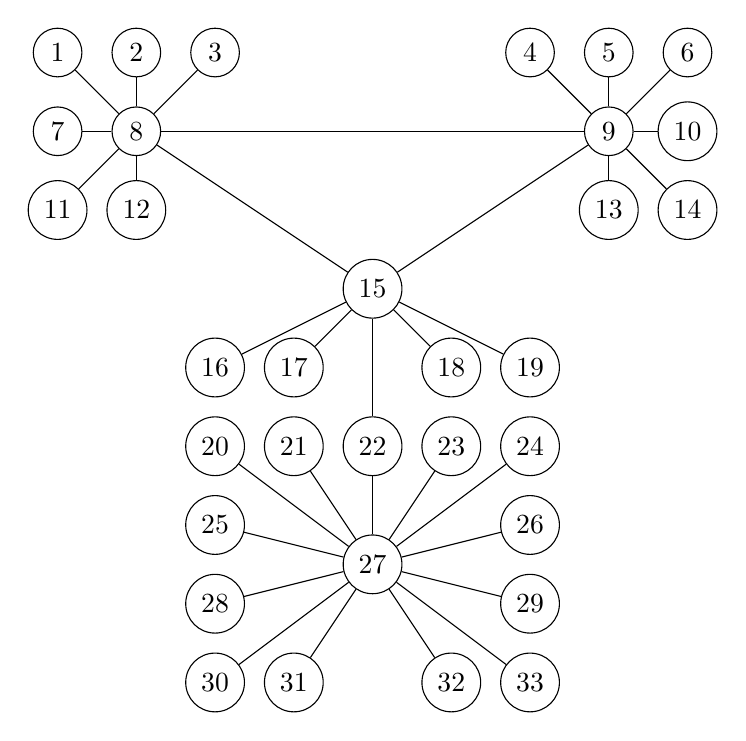
\begin{tikzpicture}
	\path 	
			% Nodos
			(0,8) node [shape=circle, draw] (1) {1}
			(1,8) node [shape=circle, draw] (2) {2}
			(2,8) node [shape=circle, draw] (3) {3}
			(6,8) node [shape=circle, draw] (4) {4}
			(7,8) node [shape=circle, draw] (5) {5}
			(8,8) node [shape=circle, draw] (6) {6}
			(0,7) node [shape=circle, draw] (7) {7}
			(1,7) node [shape=circle, draw] (8) {8}
			(7,7) node [shape=circle, draw] (9) {9}
			(8,7) node [shape=circle, draw] (10) {10}
			(0,6) node [shape=circle, draw] (11) {11}
			(1,6) node [shape=circle, draw] (12) {12}
			(7,6) node [shape=circle, draw] (13) {13}
			(8,6) node [shape=circle, draw] (14) {14}
			(4,5) node [shape=circle, draw] (15) {15}
			(2,4) node [shape=circle, draw] (16) {16}
			(3,4) node [shape=circle, draw] (17) {17}
			(5,4) node [shape=circle, draw] (18) {18}
			(6,4) node [shape=circle, draw] (19) {19}
			(2,3) node [shape=circle, draw] (20) {20}
			(3,3) node [shape=circle, draw] (21) {21}
			(4,3) node [shape=circle, draw] (22) {22}
			(5,3) node [shape=circle, draw] (23) {23}
			(6,3) node [shape=circle, draw] (24) {24}
			(2,2) node [shape=circle, draw] (25) {25}
			(6,2) node [shape=circle, draw] (26) {26}
			(4, 1.5) node [shape=circle, draw] (27) {27}
			(2,1) node [shape=circle, draw] (28) {28}
			(6,1) node [shape=circle, draw] (29) {29}
			(2,0) node [shape=circle, draw] (30) {30}
			(3,0) node [shape=circle, draw] (31) {31}
			(5,0) node [shape=circle, draw] (32) {32}
			(6,0) node [shape=circle, draw] (33) {33};
			% Aristas de la semiestrella superior izq
			\draw[-] (1) -- (8);
			\draw[-] (2) -- (8);
			\draw[-] (3) -- (8);
			\draw[-] (7) -- (8);
			\draw[-] (11) -- (8);
			\draw[-] (12) -- (8);

			% Aristas de la semiestrella superior izq
			\draw[-] (4) -- (9);
			\draw[-] (5) -- (9);
			\draw[-] (6) -- (9);
			\draw[-] (10) -- (9);
			\draw[-] (13) -- (9);
			\draw[-] (14) -- (9);

			% Mas aristas
			
			\draw[-] (8) -- (9);
			\draw[-] (8) -- (15);
			\draw[-] (9) -- (15);
			\draw[-] (16) -- (15);
			\draw[-] (17) -- (15);
			\draw[-] (18) -- (15);
			\draw[-] (19) -- (15);
			\draw[-] (22) -- (15);

			% Aristas de la estrella inferior

			\draw[-] (20) -- (27);
			\draw[-] (21) -- (27);
			\draw[-] (22) -- (27);
			\draw[-] (23) -- (27);
			\draw[-] (24) -- (27);
			\draw[-] (25) -- (27);
			\draw[-] (26) -- (27);
			\draw[-] (28) -- (27);
			\draw[-] (29) -- (27);
			\draw[-] (30) -- (27);
			\draw[-] (31) -- (27);
			\draw[-] (32) -- (27);
			\draw[-] (33) -- (27);

			
\end{tikzpicture}
